\subsection{Why is Aging a Problem?}

\begin{frame}[c]{Corona Deaths correlate with Age}
    \large
    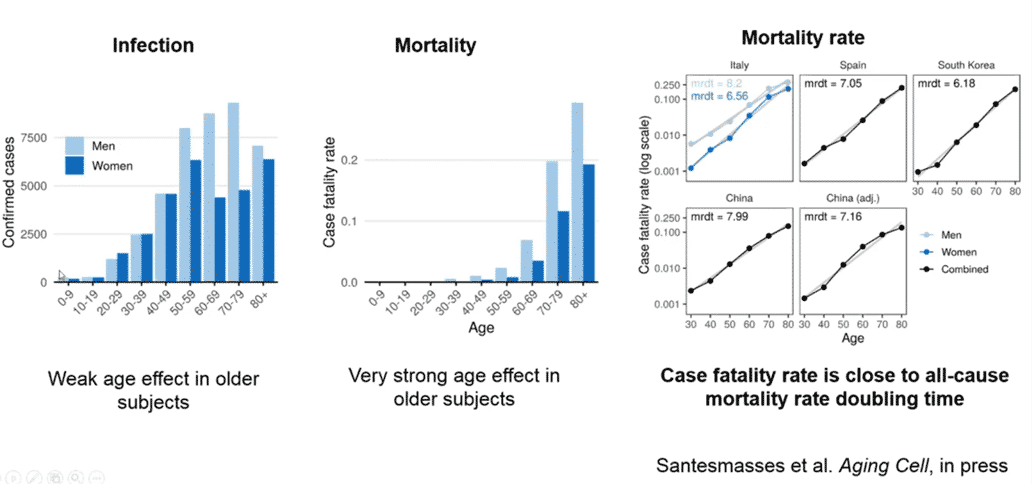
\includegraphics[width=\textwidth]{corona_death_rates} \\
    Source: \cite{10.1111/acel.13230} \\
\end{frame}


\begin{frame}[c]{Treating Corona with Senolytics (anti-aging approach)}
    % trim = l b r t
    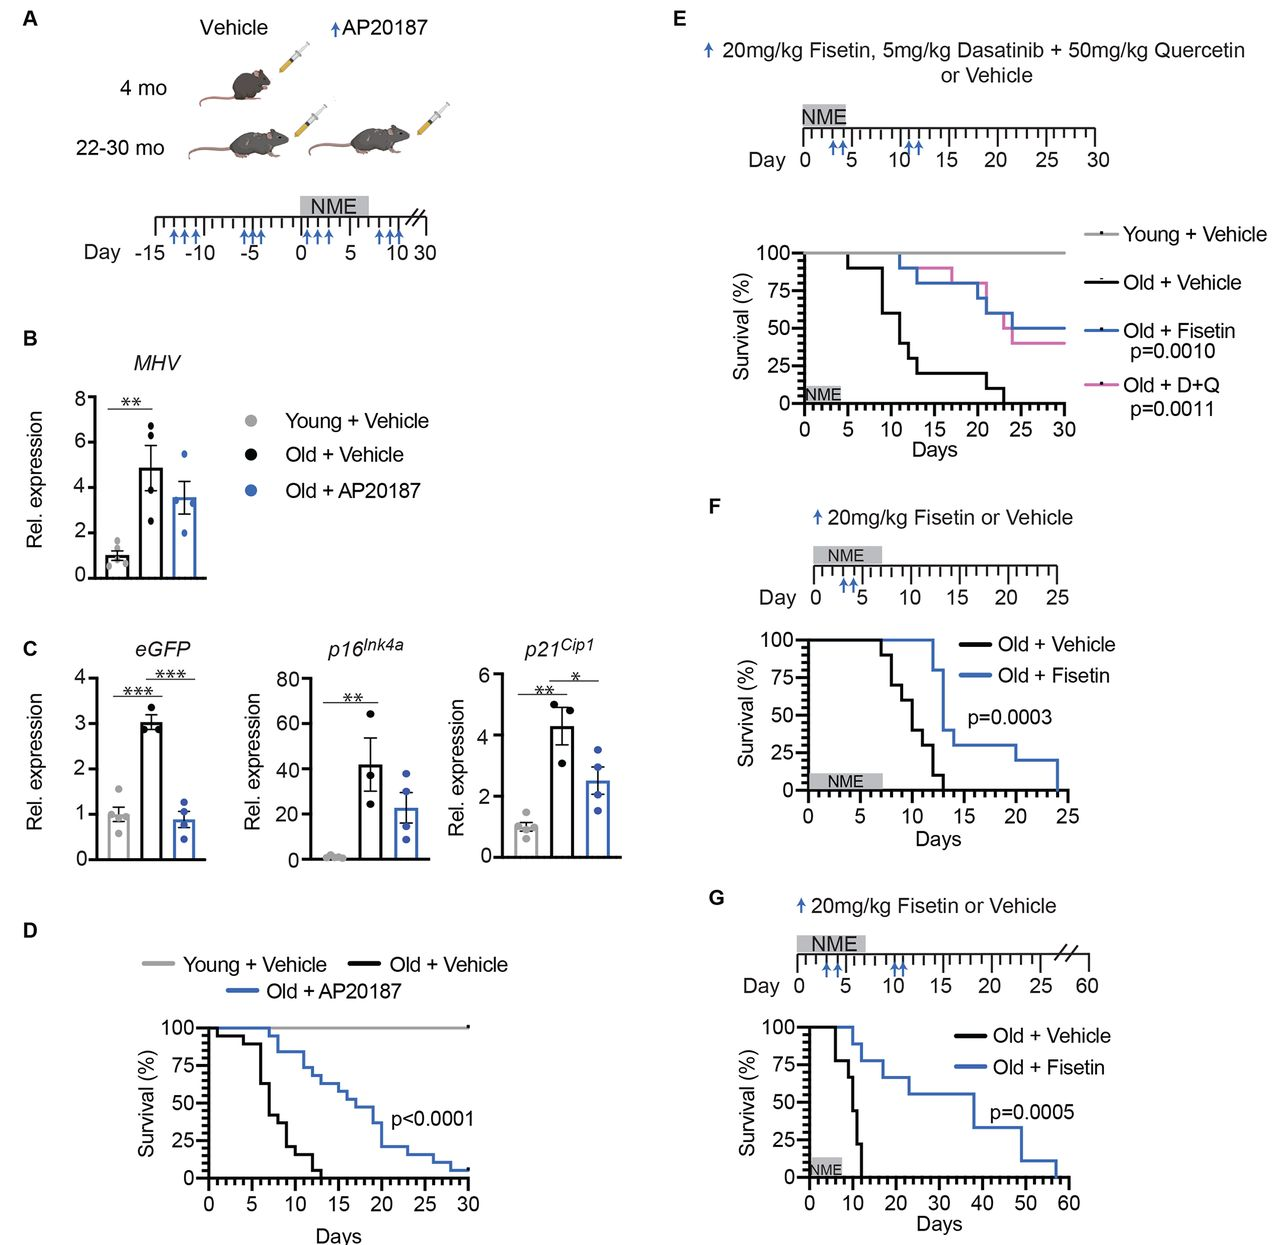
\includegraphics[width=\textwidth,clip,trim=170 180 0 50]{mice_corona} \\
    Source: \cite{camell2021senolytics} \\
    \pause
    Conclusion: They don't die due to Corona, they die due to old age!
    \pnote{Fisetin as well as Dasatinib and Quercetin are well-established senolytics}
    \pnote{NME = Normal Microbial Experience; pathogen infection/exposure}
\end{frame}


\begin{frame}[c]{All causes for Death correlate with Age}
    \large
    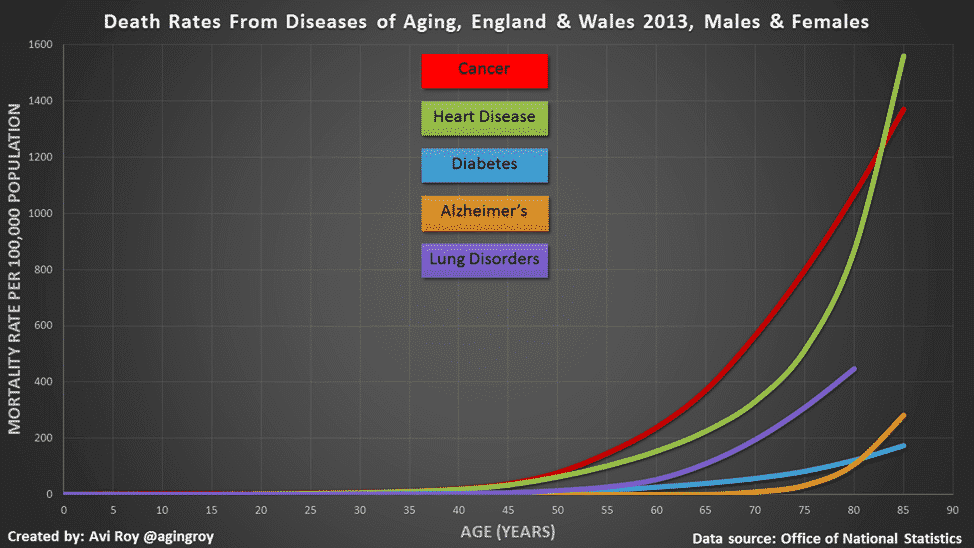
\includegraphics[width=\textwidth]{death_rates} \\
    \pause
    Same with all other primary causes!
\end{frame}


\begin{frame}[c]{Slowing aging has incredible potential}
    \large
    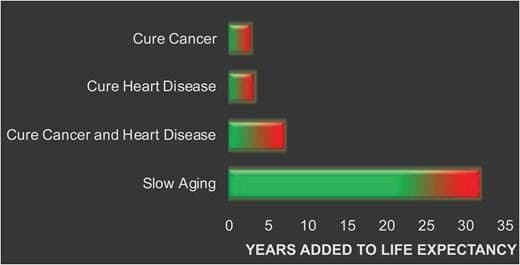
\includegraphics[width=\textwidth]{potential} \\
    Source: \cite{10.1093/ppar/prz022} \\
    \pause
    And yet it receives less than 1/100th of Funding!
\end{frame}


